\documentclass[10pt,twocolumn]{article}

% ── Packages ──────────────────────────────────────────────────────────────────
\usepackage[margin=1in, top=1in, bottom=1in]{geometry}
\usepackage{times}           % Times New Roman font, standard for CVPR
\usepackage{graphicx}
\usepackage{amsmath}
\usepackage{amssymb}
\usepackage{booktabs}
\usepackage{hyperref}
\usepackage{cite}
\usepackage{caption}
\usepackage{subcaption}
\usepackage{abstract}        % Allows styling of abstract
\usepackage{titlesec}        % Section heading control
\usepackage{fancyhdr}
\usepackage{setspace}
\usepackage{parskip}
\usepackage{algorithm}
\usepackage{algpseudocode}

% ── Page style ────────────────────────────────────────────────────────────────
\pagestyle{fancy}
\fancyhf{}
\renewcommand{\headrulewidth}{0pt}
\fancyfoot[C]{\thepage}

% ── Section heading style (bold, slightly smaller than default) ───────────────
\titleformat{\section}{\normalfont\large\bfseries\centering}{\thesection.}{0.5em}{}
\titleformat{\subsection}{\normalfont\normalsize\bfseries}{\thesubsection.}{0.5em}{}
\titleformat{\subsubsection}{\normalfont\normalsize\bfseries\itshape}{\thesubsubsection.}{0.5em}{}

% ── Abstract styling ─────────────────────────────────────────────────────────
\renewcommand{\abstractnamefont}{\normalfont\large\bfseries\centering}
\renewcommand{\abstracttextfont}{\normalfont\small\itshape}

% ── Spacing ───────────────────────────────────────────────────────────────────
\setlength{\columnsep}{0.3in}
\setlength{\parindent}{1em}
\setlength{\parskip}{2pt}

% ── Title block ───────────────────────────────────────────────────────────────
\title{%
    \vspace{-1em}
    \Large\textbf{Final Project Report} \\[0.5em]
    \normalsize
    Henry Paproski \quad Johnny Zhang \\[0.3em]
    \small
    Faculty of Science, University of Alberta \\
    \texttt{\{hpaprosk, author2\}@ualberta.ca}
}
\date{}

% ══════════════════════════════════════════════════════════════════════════════
\begin{document}

\maketitle
\thispagestyle{fancy}

% ── Abstract ──────────────────────────────────────────────────────────────────
\begin{abstract}
Lorem ipsum dolor sit amet, consectetur adipiscing elit, sed do eiusmod tempor incididunt ut labore et dolore magna aliqua.
\end{abstract}

% ── 1. Introduction ───────────────────────────────────────────────────────────
\section{Introduction}

Lorem ipsum dolor sit amet, consectetur adipiscing elit, sed do eiusmod tempor incididunt ut labore et dolore magna aliqua.

% ── 2. Related Work ───────────────────────────────────────────────────────────
\section{Related Work}

The inspiration for this project is the work presented in \cite{newcombe2010}, which introduces a method for generating dense 3D reconstructions by leveraging a sparse base produced using structure-from-motion (SfM). The appeal of this approach is the ability to take a coarse initial model and iteratively refine it into a high accuracy final model. Our implementation focuses on the core pipeline described in this system, specifically the transition from sparse mapping to dense surface estimation through scene-flow updates computed using view-predictive optical flow.

A critical component of monocular reconstruction is the underlying tracking and mapping system. The original system in \cite{newcombe2010} utilizes Parallel Tracking and Mapping (PTAM) \cite{PTAM} to provide real-time camera poses and a sparse point cloud. However, due to the limited availability of PTAM implementations compatible with Python, we substituted this component with ColMap \cite{COLMAP}, another SfM library which was readily availanle. While ColMap is typically used for offline processing, it provides the sparse foundation necessary to test the subsequent dense reconstruction stages.

The methods for dense reconstruction from a single camera involved many complex optimization problems. The methods described in \cite{newcombe2010} frequently utilize Variational methods for global energy minimization, such as the TV-L1 optical flow algorithm discussed in \cite{TV-L1} and the denoising technique mentioned in \cite{newcombe2010}. These methods ensure that the final product both aligns with what's seen in  the video while still retaining smoothness. In our implementation, we utilize Poisson reconstruction \cite{Poisson} to generate a base mesh from the initial sparse data, which is then used for further refinement. Although the reference paper \cite{newcombe2010} emphasizes live performance, our project prioritizes the algorithmic pipeline's ability to enhance model fidelity and photo-consistency by building upon existing SfM data.

% ── 3. Methods ────────────────────────────────────────────────────────────────
\section{Methods}

Our project implementation is split into seven pipeline stages. First, we use SfM to obtain a sparse point cloud and camera matrices. Second, we generate a base mesh via Poisson reconstruction. Third, we perform keyframe selection to establish bundles for refinement. Fourth, we predict views from the current mesh to analyze discrepancies using optical flow. Fifth, we update mesh vertices based on these flow results to refine the reconstruction. Sixth, we apply a denoising algorithm to ensure spatial smoothness. Finally, we integrate the refined output into a global representation of the entire scene.

\subsection{Overview}

Lorem ipsum dolor sit amet, consectetur adipiscing elit.

\subsection{Sub-method A}

Lorem ipsum dolor sit amet, consectetur adipiscing elit.

\subsection{View-Predictive Optical Flow}
\subsubsection{View-Prediction}
The purpose of the view prediction stage is to generate a virtual image that represents how a scene should appear from the perspective of a specific comparison camera, given our current 3D reconstruction. Following the methodology in [1], this "synthetic" view serves as a intermediate step for computing view-predictive optical flow. By comparing the predicted image with the actual captured image from the comparison pose, the system can identify discrepancies caused by inaccuracies in the base mesh.

Unlike the implementation described in [1], wherein the reference frame image is back-projected onto the base model, then said textured model is projected into the reference. We instead use the base mesh to obtain a depth map for the comparison frame and use it to restore the 3D coordinates where each ray in the image intersects the base mesh and project those points into the reference frame. Once we do that we have a map for which pixel in the reference corresponds to a given pixel in the comparison so we perform a sampling to obtain our final image prediction. This process is shown in more detail in algorithm 1.

\begin{algorithm}
\caption{View-Predictive Image Synthesis}
\begin{algorithmic}[1]
\State $K_{inv} \leftarrow K^{-1}$
\For{each pixel $\mathbf{u} = (x, y)$ in comparison frame}
    \State $\mathbf{r} \leftarrow K_{inv} \cdot \tilde{\mathbf{u}}$
        \Comment{Back-project to camera ray}
    \State $\hat{\mathbf{r}} \leftarrow \mathbf{r} / \|\mathbf{r}\|$
    \State $X_{comp} \leftarrow \hat{\mathbf{r}} \cdot D(\mathbf{u})$
        \Comment{Scale by Euclidean depth}
    \State $X_{world} \leftarrow R_{comp}^{-1}(X_{comp} - t_{comp})$
    \State $X_{ref} \leftarrow R_{ref} \cdot X_{world} + t_{ref}$
    \State $\tilde{\mathbf{u}}_{ref} \leftarrow K \cdot X_{ref}$
        \Comment{Project into reference}
    \State $\mathbf{u}_{ref} \leftarrow \tilde{\mathbf{u}}_{ref} / X_{ref}[2]$
        \Comment{Dehomogenise}
    \If{$\mathbf{u}_{ref}$ inside image bounds \textbf{and} $X_{ref}[2] > 0$}
        \State $I_{pred}(\mathbf{u}) \leftarrow I_{ref}(\mathbf{u}_{ref})$
    \Else
        \State $I_{pred}(\mathbf{u}) \leftarrow 0$
            \Comment{Mark invalid}
    \EndIf
\EndFor
\State \Return $I_{pred}$
\end{algorithmic}
\end{algorithm}

Unfortunately, in cases where the pixels land outside of the image boundary or there is no base mesh we are unable to extract any information about said pixel and simply set it to zero as seen in figure 1. To keep track of these pixels we actually construct a mask of valid pixels, which simply tells us which pixels didn't intersect the base mesh and which pixels mapped to someplace that was outside of the reference image boundaries.

\begin{figure}[h]
    \centering
    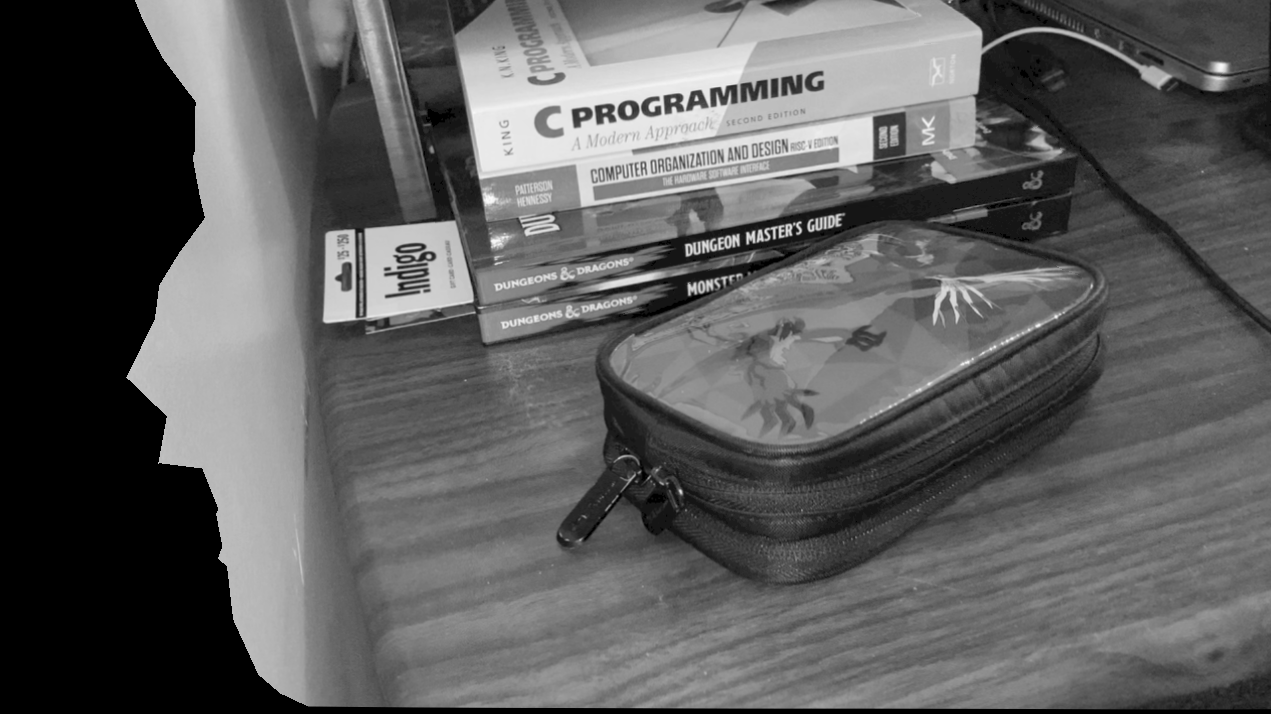
\includegraphics[width=\columnwidth]{predicted_0.png}
    \caption{An Image prediction generated using algorithm 1}
    \label{fig:your_label}
\end{figure}

\subsubsection{Optical Flow}

Dense correspondence between the reference and comparison frames is the core mechanism by which the base mesh is refined. Following Newcombe and Davison \cite{newcombe2010}, we compute optical flow not between raw image pairs, but between a synthesized view prediction and the true comparison image. Because the view prediction already accounts for the rotational component of camera motion, the residual flow field measures only the geometric error in the current mesh estimate, dramatically reducing the displacement magnitudes that the flow algorithm must handle.

The flow is computed by minimizing the TV-L$^1$ energy function \cite{wedel2009}:

\begin{equation}
    \mathbf{E_u} = \int_\Omega \lambda |I_0(\mathbf{x}) - I_1(\mathbf{x} + \mathbf{u}(\mathbf{x}))| \, d\mathbf{x} + \int_\Omega |\nabla \mathbf{u}| \, d\mathbf{x}
\end{equation}

where $I_0$ and $I_1$ are the image pair, $\mathbf{u}$ is the displacement field, and $\lambda$ provides a trade-off between the data fidelity and regularization term. The data term provides robustness to image data errors, and the regularization allows flow discontinuities at occlusion boundaries while producing smooth fields elsewhere \cite{newcombe2010}.


The minimization of this function is done using the method described in \cite{wedel2009}. Wherein they define an auxiliary variable $\mathbf{v}$, and use the following convex approximation to solve for \(d\) dimensional TV-L$^1$:

\begin{equation}
\mathbf{E_\theta}=\int_\Omega \{\sum_d |\nabla u_d|+\sum_d\frac{1}{2\theta}(u_d-v_d)^2+\lambda|\rho(v)| \}
\end{equation}

Where \(\theta\) is a small constant such that v is a sufficiently close approximation of u and \(\rho\) denotes the image residual. Additionally, in the case of optical flow, $\mathbf{u}$ only has 2 dimensions and thus d in this case is 2. From this convex approximation, a solution can be obtained by performing alternating updates to $\mathbf{u}$ and $\mathbf{v}$.

To update $\mathbf{v}$ let $\rho(\mathbf{u}) = I_1(\mathbf{x} + \mathbf{u}_0) + \nabla I_1 \cdot (\mathbf{u} - \mathbf{u}_0) - I_0(\mathbf{x})$ and define the threshold $\kappa = \lambda \theta |\nabla I_1|^2$. The point-wise update for $\mathbf{v}$ is then:
\begin{equation}
\mathbf{v} = \mathbf{u} + 
\begin{cases} 
\lambda \theta \nabla I_1 & \text{if } \rho(\mathbf{u}) < -\kappa \\
-\lambda \theta \nabla I_1 & \text{if } \rho(\mathbf{u}) > \kappa \\
-\rho(\mathbf{u}) \frac{\nabla I_1}{|\nabla I_1|^2} & \text{if } |\rho(\mathbf{u})| \leq \kappa
\end{cases}
\end{equation}

Once $\mathbf{v}$ is updated, we then perform an update for $\mathbf{u}$ using a dual formulation, with a dual variable $\mathbf{p}$, as follows:
\begin{align}
    \mathbf{p}^{k+1} &= \frac{\mathbf{p}^k + (\tau/\theta) \nabla \mathbf{u}^k}{1 + (\tau/\theta) |\nabla \mathbf{u}^k|} \\
    \mathbf{u}^{k+1} &= \mathbf{v} + \theta \text{div}(\mathbf{p}^{k+1})
\end{align}
where $\tau \leq 1/8$ is the step size. This procedure is only valid for small displacements, and thus is embedded within a coarse-to-fine image pyramid, which will help in avoiding convergence to unfavorable local minima.

\subsubsection{Structure-Texture Decomposition}

A known limitation of intensity-based optical flow is its sensitivity to illumination artifacts such as shadows and shading reflections, which violate the brightness constancy assumption. To address this, we apply a structure-texture decomposition to both the predicted and comparison images before computing flow. The decomposition separates each image into a structural component $I_S$, corresponding to the large-scale geometry of the scene, and a texture component $I_T = I - I_S$, containing fine-scale detail from which illumination artifacts have been largely removed as seen in figure 2. As shown in Wedel et al.\ \cite{wedel2009}, computing flow on the texture component yields substantially more accurate estimates in the presence of shadows and reflections. In our implementation, this decomposition is computed using a skimage library, and the texture images are passed to the flow computation in place of the originals.

\begin{figure}[h]
    \centering
    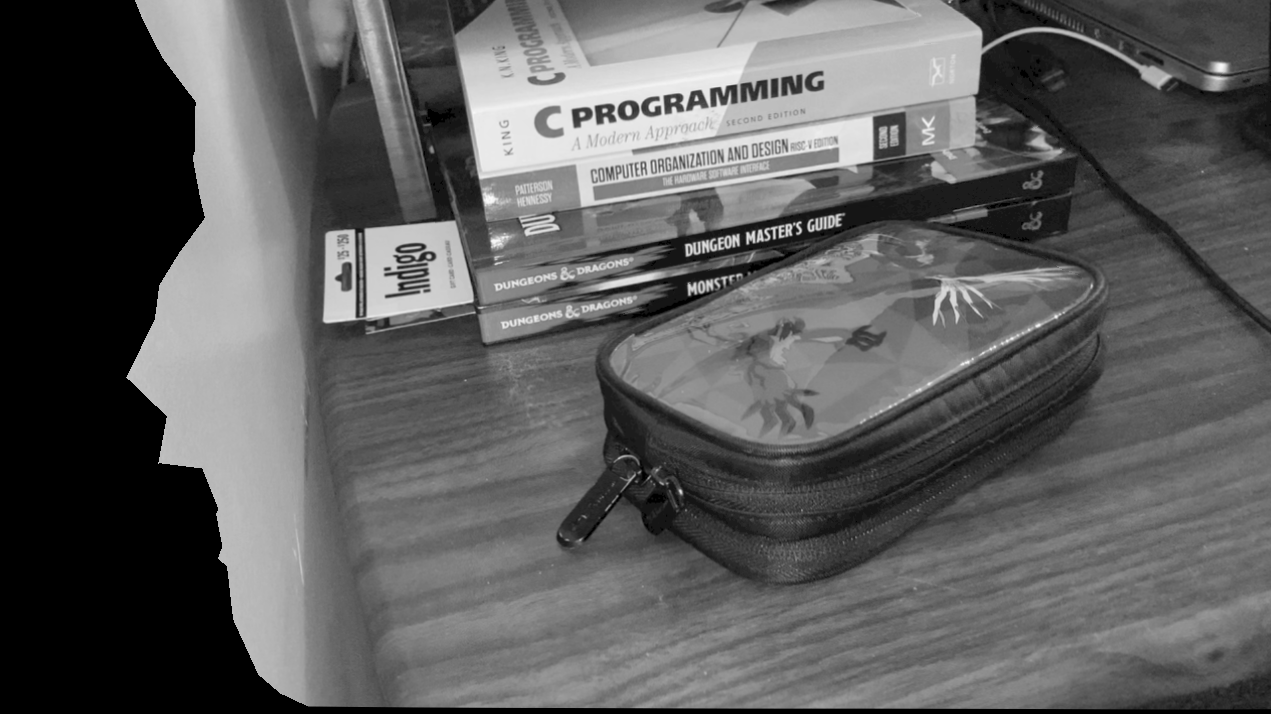
\includegraphics[width=\columnwidth]{predicted_0.png}
    \caption{An Image prediction generated using algorithm 1}
    \label{fig:your_label}
\end{figure}

\subsubsection{Forward-Backward Consistency}

Optical flow estimation is inherently unreliable in occluded regions, where a pixel visible in one frame has no correspondence in the other. To discard such unreliable flow vectors before they influence the scene flow update, we apply a forward-backward consistency check. For each pixel, we compute the forward flow $\mathbf{u}_{fwd}$ from the predicted image to the comparison image, and the backward flow $\mathbf{u}_{bwd}$ in the reverse direction. When there is no occlusion, and the optic flow is accurate the backward flow should point in the opposite direction of the forward flow: $\mathbf{u}_{fwd}(\mathbf{x}) + \mathbf{u}_{bwd}(\mathbf{x} + \mathbf{u}_{fwd}(\mathbf{x}))=0$. Let $\mathbf{w}(\mathbf{x})=\mathbf{u}_{bwd}(\mathbf{x} + \mathbf{u}_{fwd}(\mathbf{x}))$, then a pixel's flow is marked valid only if this value falls below an adaptive threshold proportional to the local flow magnitude as follows:
\begin{equation}
|\mathbf{u}_{fwd}(\mathbf{x}) + \mathbf{w}(\mathbf{x})|^2 \lt 0.01(|\mathbf{u}_{fwd}|^2+|\mathbf{w}(\mathbf{x})|^2)+0.5
\end{equation}

This approach, motivated by the occlusion reasoning in \cite{sundaram2010}, ensures that flow vectors in occluded or poorly constrained regions, such as those which are close to black regions generated by holes in the base mesh, are zeroed out before contributing to the depth update, preventing noisy $\lambda_j$ estimates from corrupting the mesh refinement. 

% ── 4. Experiments ────────────────────────────────────────────────────────────
\section{Experiments}

Lorem ipsum dolor sit amet, consectetur adipiscing elit, sed do eiusmod tempor incididunt ut labore et dolore magna aliqua.

\subsection{Dataset and Setup}

Lorem ipsum dolor sit amet, consectetur adipiscing elit.

\subsection{Results}

Lorem ipsum dolor sit amet, consectetur adipiscing elit.

% ── 5. Conclusions ────────────────────────────────────────────────────────────
\section{Conclusions}

Lorem ipsum dolor sit amet, consectetur adipiscing elit, sed do eiusmod tempor incididunt ut labore et dolore magna aliqua.

% ── Acknowledgements (optional) ───────────────────────────────────────────────
\section*{Acknowledgements}

Lorem ipsum dolor sit amet, consectetur adipiscing elit.

% ── References ────────────────────────────────────────────────────────────────
\section*{References}

% Option A: manual references (matching the plain numbered style of the paper)
\begingroup
\renewcommand{\section}[2]{}   % suppress duplicate "References" heading from bibliography
\small
\begin{thebibliography}{99}

\bibitem{newcombe2010}
R.~A. Newcombe and A. J. Davison.
\newblock Live dense reconstruction with a single moving camera.
\newblock \textit{Proceedings of the IEEE Conference on Computer Vision and Pattern Recognition (CVPR)}, 2010.

\bibitem{PTAM}
G.~Klein and D.~Murray.
\newblock Parallel tracking and mapping for small AR workspaces.
\newblock \textit{Proceedings of the International Symposium on Mixed and Augmented Reality (ISMAR)}, 2007.

\bibitem{COLMAP}
J.~L. Schönberger and J.~M. Frahm.
\newblock Structure-from-motion revisited.
\newblock \textit{Proceedings of the IEEE Conference on Computer Vision and Pattern Recognition (CVPR)}, 2016.

\bibitem{TV-L1}
C.~Zach, T.~Pock, and H.~Bischof.
\newblock A duality based approach for realtime TV-L1 optical flow.
\newblock \textit{Proceedings of the Joint Pattern Recognition Symposium}, 2007.

\bibitem{Poisson}
M.~Kazhdan, M.~Bolitho, and H.~Hoppe.
\newblock Poisson surface reconstruction.
\newblock \textit{Proceedings of the Eurographics Symposium on Geometry Processing (SGP)}, 2006.

\bibitem{wedel2009}
A.~Wedel, T.~Pock, C.~Zach, H.~Bischof, and D.~Cremers.
\newblock An improved algorithm for {TV-L1} optical flow.
\newblock In \textit{Proceedings of the Dagstuhl Seminar on Statistical and Geometrical Approaches to Visual Motion Analysis}, pages 23--45, 2009.

\bibitem{sundaram2010}
N.~Sundaram, T.~Brox, and K.~Keutzer.
\newblock Dense point trajectories by {GPU}-accelerated large displacement optical flow.
\newblock In \textit{Proceedings of ECCV}, pages 438--451, 2010.

\end{thebibliography}
\endgroup

\end{document}
